\documentclass{article}
\usepackage[english]{babel} % en
\usepackage{graphicx}
\usepackage{hyperref}
\usepackage[T1]{fontenc}
\usepackage[utf8]{inputenc}
\usepackage{setspace}
\usepackage[paper=a4paper,margin=1in]{geometry}
\usepackage{parskip}
\usepackage{fancyhdr}
\usepackage{cite}
\usepackage{units}
\usepackage[htt]{hyphenat}
\usepackage{enumitem}
\usepackage{wrapfig}
\usepackage{mathtools}
\usepackage{relsize}
\usepackage{listings}
\usepackage{xcolor}
\usepackage{amsfonts}

\graphicspath{{./images/}}

\title{\textbf{Discrete Logarithm: ElGamal, Algorithms, Practice}  \\[0.4em] \smaller{} Seminar in Algebraic Methods and Algorithms in Cryptology}
\author{Ilaria Battiston}
\date{Summer Semester 2020}
\pagestyle{fancy}

\begin{document}
	
	\maketitle
	
	\lfoot{}
	\cfoot{}
	\rfoot{\thepage}
	
	\newpage
	\setcounter{tocdepth}{2}
	\tableofcontents
	\newpage
	
	\section{Introduction}
A \textbf{cryptosystem} consists of a family of \textit{enciphering transformations} $f$, each corresponding to a choice of parameters $p$, from a set $P$ of all possible plaintext message units to a set $C$ of all possible ciphertext message units. The transformation requires:
\begin{itemize}
	\item An algorithm, which is the same for the whole family and supposedly publicly known;
	\item An enciphering key $K_E$, the value of parameters $p$;
	\item A deciphering key $K_D$.
\end{itemize}
The deciphering key is needed in order to compute $f^{-1}$, i.e.\ decipher the message. The transformation uses the same algorithm as encrypting, except with a different key. 

A \textbf{public key} or \textbf{asymmetric cryptosystem}, by definition, has the property that someone who knows only to encipher cannot use the encipher key to find the deciphering key without a prohibitively lengthy computation: the function $f : P \rightarrow C$ is easy to compute once $K_E$ is known, but it is very hard in practice to compute the inverse function $f^{-1} : C \rightarrow P$.

In mathematical terms, the inverse computation should be \textbf{infeasible}, namely so computationally intensive that it is impossible to evaluate it in any reasonable time period. 

This implies that $f$ is not invertible without some additional information, therefore $f$ is an \textit{one-way function}. Most public key algorithms are in fact based on number-theoretic functions, whose goal is usually not to have a compact mathematical description between input and output.

A public key cryptosystem, therefore, involves not only one key but a pair: one is public and can be publicly shared, and the other is private and its discover by a third part would compromise the security of the system.

The main point of this scheme is that it is not necessary that the key possessed by the person who encrypts the message is secret. Receivers can only decrypt using their secret key.

Information needed to send secret messages, therefore, can be made public without anyone being able to read the content. This makes communication possible within two parts which have never interacted before, an useful feature among modern systems with huge workloads. 

\subsection{Cyclic groups and generators}
\textbf{Cyclic groups} are a way to generalize public key algorithms within groups not necessarily constrained by a prime number. They have a key role in cryptography, since they allow many useful one-way functions which can be used to encrypt information: in fact, cryptographic functions which are hard to break should be defined within finite groups.

A \textbf{group} is a set of elements $G$ together with an operation $\circ$ which combines two elements of $G$. A group has the following properties:
\begin{enumerate}
	\item The group operation $\circ$ is \textit{closed}: for all $a, b \in G$, it holds that $a \circ b = c \in G$;
	\item The group operation is \textit{associative}: $a \circ (b \circ c) = (a \circ b) \circ c$ for all $a, b, c \in G$;
	\item There is an element $1 \in G$ called the \textit{neutral element} (identity) such that $a \circ 1 = 1 \circ a = a$ for all $a \in G$;
	\item For each $a \in G$ there exists an element $a^{-1}$ called the \textit{inverse}, such that $a \circ a^{-1} = a^{-1} \circ a = 1$;
	\item A group $G$ is \textit{abelian} (or \textit{commutative}) if, furthermore, $a \circ b = b \circ a$ for all $a, b \in G$.
\end{enumerate}
Cryptography majorly relies on \textit{multiplicative groups}, where the operation $\circ$ denotes multiplication.

Algorithms related to discrete logarithm problem, for example, concern the group $\mathbb{Z}^*_n$, consisting in the set of all integers $i = 0, 1, \dots, n - 1$ for which $\gcd(i, n) = 1$. $\mathbb{Z}^*_n$ forms an abelian group under multiplication modulo $n$, where the identity element is $e = 1$.

Since cryptography concerns finite structures, groups also have to respect the property to have a finite number of elements, defining the \textit{cardinality} or \textit{order} of the group $G$ by $|G|$. 

Every element of a group $G$ has also an order, which is the smallest positive integer $k$ such that:
$$a^k = a \circ a \circ \dots \circ a = 1$$
The $\circ$ operation is applied $k$ times, obtaining the identity element of $G$.

Example: the order of the element $a = 3$ in the group $\mathbb{Z}^*_{11}$ is 5, since $a^5 = 1 \mod 11$. 

The powers of $a$ run through the same finite sequence of remainders indefinitely, adopting a cyclic behavior. This allows to introduce cyclic groups.

A group $G$ which contains an element $\alpha$ with maximum order $|G|$ is said to be \textbf{cyclic}. Elements with maximum order are called primitive or \textbf{generators}, since every element $a$ of $G$ can be written as a power $\alpha^i = a$ of this element for some $i$, so that $\alpha$ generates the entire group.

For every prime $p$, $(\mathbb{Z}^*_p, \cdot)$ is an abelian finite cyclic group.

Having a finite cyclic group $G$, some interesting properties hold:
\begin{enumerate}
	\item For every $a \in G$, it holds that:
	\begin{enumerate}
		\item $a^{|G|} = 1$;
		\item The order of $a$ divides $|G|$;
	\end{enumerate}
	\item The number of primitive elements of $G$ is $\phi(G)$, where $\phi$ defines the Euler function (number of positive integers up to $G$ which are coprime to it);
	\item if $|G|$ is prime, then all elements $a \neq 1$ are primitive.
\end{enumerate}
Those concepts have relevancy in cryptography: prime fields are widely used for building discrete logarithm cryptosystems, using the fact that in a cyclic group \textit{only element orders which divide the group cardinality} exist. 

\subsubsection{Subgroups}
\textbf{Subgroups} are subsets of cyclic groups which are groups themselves, therefore respect all the previously stated properties. 

Let $(G, \circ)$ be a cyclic group. Then, every element $a \in G$ with $ord(a) = s$ is the primitive element of a cyclic subgroup with $s$ elements.

As previously stated, the generator can be non-unique. An important special case are subgroups of prime order: with cardinality $q$, all elements $e \neq 1$ have order $q$ as well.

If $H$ is a subgroup of $G$, then $|H|$ divides $|G|$. 

To obtain a construction method for subgroups from a given finite cyclic group, only the cardinality $n$ and a primitive element are needed: then, $\alpha^{n/k}$ is computed to obtain a generator $\alpha$ of the subgroups with $k$ elements.

This follows knowing that every integer $k$ which divides the cardinality $n$ there exists exactly one cyclic subgroup $H$ of $G$ of order $k$, consisting in the elements $a \in G$ satisfying $a^k = 1$. 



	\section{The Discrete Logarithm problem}
The \textbf{discrete logarithm} cryptosystem was proposed in the mid-1970s, and to this day there are no deterministically successful known attacks against it if the parameters are chosen carefully. It is the base of several public key cryptosystems taking advantage of its computational difficulty.

It is a public-key cryptography algorithm which can be used for encryption, integrity check and digital signatures, binding the key to an identity. It works taking advantage of the properties of mathematical operations within groups.

\textit{If $G$ is a finite group, $b$ is an element of $G$, and $y$ is an element of $G$ which is a power of $b$, then the discrete logarithm of $y$ to the base $b$ is any integer $x$ such that $b^x = y$.}

Applying this statement to the finite cyclic group $\mathbb{Z}^*_p$ of order $p - 1$, taking a primitive element $\alpha \in\mathbb{Z}^*_p$ and another element $\beta \in \mathbb{Z}^*_p$, the discrete logarithm problem aims to determine the integer $1 \leq x \leq p - 1$ such that:
$$\alpha^x \equiv \beta \mod p \qquad \rightarrow \qquad x = \log_\alpha\beta \mod p$$

The discrete logarithm cryptosystem, as previously stated, relies on the fundamental fact that raising a number $b$ to a power $x$ in a large finite field is an one-way function, i.e.\ it is far more difficult to apply the inverse operation and finding $\log_bx$. 

Since the domain is a finite group, such as $\mathbb{Z}^*_n$, the repeated-squaring method can be used to compute $b^x$ with time polynomial in $\log x$, but given an element $y = b^x$, finding $y$ is an open problem.

\subsection{Example}
This example considers a discrete logarithm in the group $\mathbb{Z}^*_{47}$, in which $\alpha = 5$ is a primitive element. The problem consist in finding the positive integer $x$ such that $5^x \equiv 41 \mod 47$.

Even for small numbers, obtaining this value is not immediate. A brute-force attack, i.e.\ systematically trying all possible values for $x$, reveals that the result is $x = 15$.

$\mathbb{Z}^*_{47}$ has order 46, which implies that its subgroups have cardinality of 23, 2 and 1. $\alpha = 2$ is an element with 23 elements, and since 23 is prime then $\alpha$ is primitive. Using prime cardinality is important in order to avoid potential attacks.

When a number $a$ is not a primitive element but another generator for reasonably small $n$, computing the discrete logarithm is still doable solving a system of linear congruences.

\subsection{Generalized discrete logarithm}
Despite prime multiplicative groups increment security, the discrete logarithm applications are not limited to them and can be defined over \textit{any cyclic group}.

Given a finite cyclic group $G$ with an operation $\circ$ and cardinality $n$, having a primitive element $\alpha \in G$ and another element $\beta \in G$, the generalized discrete logarithm problem is finding the integer $1 \leq x \leq n$ such that:
$$\beta = \alpha \circ \alpha \circ \dots \circ \ alpha = \alpha^x$$

$x$ always exists in both cases with $p$ and $n$, since $\alpha$ is a primitive element and can generate every other component. 

However, there are cyclic groups in which cracking discrete logarithm is not difficult, since the function is not a one-way. For instance, in $G = (\mathbb{Z}_{11}, +)$ with primitive element $\alpha = 2$, the term $x$ for $\beta = 3$ can be computed with the following steps:
\begin{enumerate}
	\item Expressing the operation as multiplication, $x \cdot 2 \equiv 3 \mod 11$;
	\item Inverting the primitive element $\alpha$, resulting in $x \equiv 2^{-1}3 \mod 11$;
	\item Computing $2^{-1} \equiv 6 \mod 11$;
	\item Obtaining $x \equiv 2^{-1}3 \equiv 7 \mod 11$.
\end{enumerate}
This procedure can be generalized to any additive group for arbitrary $n$ and $\alpha, \beta \in \mathbb{Z}_n$, making the \textbf{generalized discrete logarithm} computationally easy over $\mathbb{Z}_n$ since there are mathematical operations which are not in the additive group (inversion, multiplication). 

Strong groups in which discrete logarithm can be used in practice to encrypt data are instead $\mathbb{Z}_p$ or the cyclic group formed by an elliptic curve.

\subsection{Computational aspects}
Despite the discrete logarithm being a strong encryption system, it requires strict constraints to be met regarding fields, length of involved factors, as well as a relevant number of exponentiation, an operation known to be expensive.

An undesired consequence of the long operands of discrete logarithm is that computation is extremely arithmetically intensive: it is not uncommon that one public key operation is by 2-3 orders of magnitude slower than using a private key system. 

Since the numbers involved are large, it is more efficient to reduce to modulo multiple times during the computation, with a process called modular exponentiation which relies on the Euclidean algorithm, usually a built-in function of modern programming languages. 

On modern computers, such execution procedures are common, and do not consist in a problem, yet performance can be a serious bottleneck in constrained devices with small CPUs.

\subsection{Security and NP-completeness}
Since public key algorithms are based on number-theoretic functions, one distinguish feature of them is that they require arithmetic with very long operands and keys. An algorithm is said to have a ``security level of $n$ bits'' if the best known attack requires $2^n$ steps, since the key is $n$ bits long.

Different security levels for discrete logarithms are:
\begin{table}[h]
	\centering
	\begin{tabular}{c|c}
		\textit{Bit lengths} & \textit{Security level} \\
		\hline
		1024 bit & 80 bit \\
		\hline
		3072 bit & 128 bit \\
		\hline
		7680 bit & 192 bit \\
		\hline
		15360 bit & 256 bit
	\end{tabular}
\end{table}

In order to provide long-term security, i.e.\ ensure that the schema will not be cracked even with the computational power obtained with several decades of hardware development, a security level of at least 128 bit should be chosen. 

Despite the existence of sophisticated algorithms running faster than a brute-force approach, and even a quantum algorithm, none of them is able to run in polynomial time. 

Furthermore, efficient classical algorithms also exist in certain cases, while on the other hand there exist groups for which computing the discrete algorithm is much more difficult, therefore the domain must be chosen carefully. 

\subsection{Real-life applications}
Usage of the discrete logarithm is standardized by The Internet Key Exchange (IKE), which defines cyclic groups and their order, despite some of them being of less than 1024 bit and therefore potentially breakable. 

The European Institute for System Security has furthermore established a family of practical cryptography protocols based on discrete logarithm, which were originally intended for LAN security but quickly extended their scope: nowadays, discrete logarithm is used within implementations of access control, authentication, confidentiality protection, key exchange, digital signature and distributed network security management.

The most popular practical application of discrete logarithm is, however, the \textit{Diffie-Hellman key exchange}: since discrete logarithm needs extensive computational power and longer keys than symmetric encryption, it is mostly used for exchanging a private key in a secure way.


	\section{The Diffie-Hellman key exchange}
Since public key cryptosystems are relatively slowly compared to private key ones, it is often more realistic to use them in conjunction with classical schemes, giving them the limited role of key exchange and agreement.

A major flaw of symmetric cryptosystems, in fact, is that key establishment must be done through secure means, and \textbf{information cannot directly be sent over the channel}. The two parts must have prior knowledge and trust of each other, and cannot publicly share information. 

This can be solved encrypting a symmetric key using a public key algorithm, so that after the decryption it can be used by both parts to encrypt and decrypt using the symmetric cipher. 

The first published proposal for a \textbf{key exchange based on public cryptography} is attributed to W. Diffie and M. E. Hellman, and was based on the discrete logarithm problem.

The process involves two individuals agreeing on an arbitrary starting number which does not have to be kept secret, while each one secretly chooses another value to keep to himself. Then, the secret is mixed with the public key, and the result is exchanged. 

Finally, the received output is once again combined with the other secret, giving the original message. If a third party listened to the exchange, it would only know the common number and the mixed one, with the inability to retrieve the original value in an efficient way.

Diffie-Hellman is not an encryption algorithm, but rather a \textit{protocol} defining the necessary series of step in order to achieve the exchange of encrypted information between two parties through asymmetrical cryptography. 

The basic idea behind the Diffie-Hellman Key Exchange (DHKE) is that exponentiation in $\mathbb{Z}^*_p$ with $p$ prime is a one-way function and the exponentiation is commutative, i.e.:
$$k = (a^x)^y \equiv (a^y)^x \mod p$$

The value $k$ is the joint secret which can be used as session key between the two parties. 

The set-up protocol consists of the following steps:
\begin{enumerate}
	\item Choose a large prime $p$;
	\item Choose an integer $\alpha \in \{2, 3, \dots, p - 2\}$, which ideally should be a generator;
	\item Publish $p$ and $\alpha$ (domain parameters).
\end{enumerate}

If Alice and Bob both know the public parameters $p$ and $\alpha$, they can generate a joint secret key $k$ with the DHKE protocol:

\begin{figure}[h]
	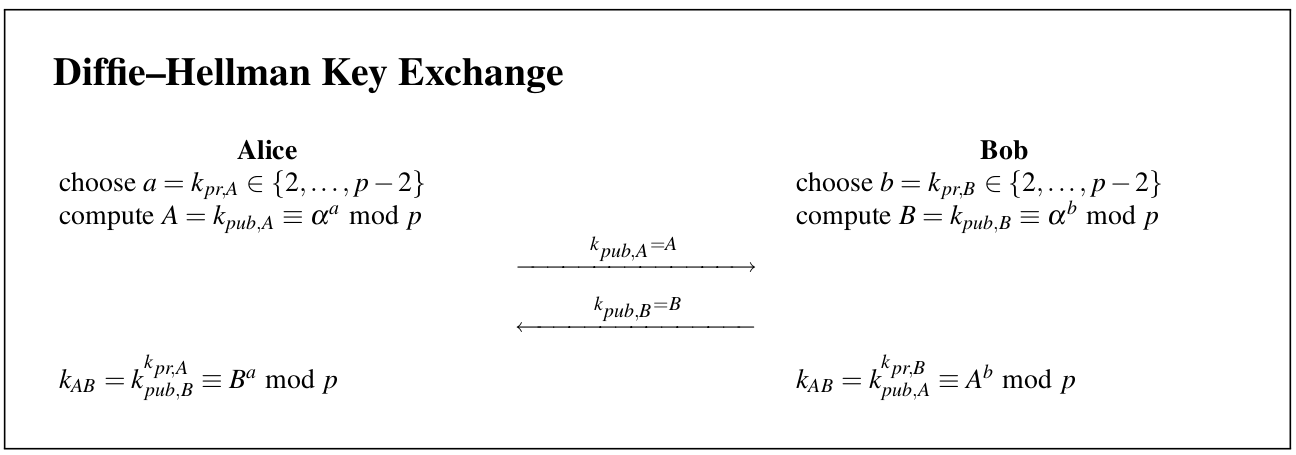
\includegraphics[scale=0.35]{DiffieHellmanPaar.png}
	\centering
\end{figure}

Enciphering and deciphering between Alice and Bob can now be performed by both parts:
$$k_{AB} = k^{k_{pr, A}}_{k_{pub, B}} \equiv B^a \mod p$$
$$k_{AB} = k^{k_{pr, B}}_{k_{pub, A}} \equiv A^b \mod p$$

The correctness of this protocol is simple to prove: 
\begin{itemize}
	\item Alice computes $B^a \equiv (\alpha^b)^a \equiv \alpha^{ab} \mod p$;
	\item Bob computes $A^b \equiv (\alpha^a)^b \equiv \alpha^{ab} \mod p$.
\end{itemize}
Now both of them share the session key $k_{AB} \equiv \alpha^{ab} \mod p$ which can be used to establish a secure connection for a symmetric algorithm. 

This protocol can also be extended with more than two parties: any number of users can take part in the exchange by performing more iterations of the algorithm and exchanging intermediate data.

\subsection{Security of Diffie-Hellman}
Basic Diffie-Hellman protocol is not secure against active attacks: messages can be either modified or falsely generated by a malicious third part, harming its security through a so called man-in-the-middle attack. 

However, if generators and finite groups are chosen carefully and large enough, the protocol is considered secure. 

Passive attacks. i.e.\ ones in which an attacker can only listen but not alter information, take place trying to compute the session key $k_{AB}$ shared between Alice and Bob. 

Just by observing the protocol, one could obtain:
\begin{itemize}
	\item $\alpha$ and $p$, since those are public parameters;
	\item Values $A = k_{pub, A}$ and $B = k_{pub, B}$ by eavesdropping on the channel during an execution of a key exchange.
\end{itemize}
The question is whether $k = \alpha^{ab}$ can be computed as well, assuming that $\alpha$, $p$, $A \equiv \alpha^a \mod p$ and $B \equiv \alpha^b \mod p$ are known.

The previously stated problem is called the Diffie-Hellman problem, and can be generalized to arbitrary finite cyclic groups.

Given a finite cyclic group $G$ of order $n$, a primitive element $\alpha \in G$ and two elements $A = \alpha^a$ and $B = \alpha^b$ in $G$, the Diffie-Hellman problem is to find the group element $\alpha^{ab}$.

One general approach to solve it consists in considering the DHP in the multiplicative group $\mathbb{Z}^*_p$, and requires an effective way to compute discrete logarithms within it. Then, the key can be found with those steps:
\begin{enumerate}
	\item Computing Alice's private key $a = k_{pr, A}$ by solving $a \equiv \log_\alpha A \mod p$;
	\item Computing the session key $k_{A, B} \equiv B^a \mod p$.
\end{enumerate}

It is unknown whether solving the DLP is the only way to crack the Diffie-Hellman protocol without computing the discrete logarithm, but at the moment this is the only available method. 

The order of the finite group cardinality should have a large prime factor $p$ to prevent usage of attacking algorithms to obtain the exponent. For this reason, so called safe primes $q$ are used to calculate $p = 2q + 1$, such that the order of the group is only divisible by 2 and $q$.

Hence, in order to ensure security in practice, there must be the assumption that this problem cannot be solved in an efficient way, choosing $p$ sufficiently large to make the computation infeasible. 

Furthermore, private keys should always stem from a true random generator in order to prevent an attacker to guess them.

$p$ is consequently generated using a probabilistic prime-finding algorithm, and should have a length of at least 1024 bits in order to provide strong security.

\subsubsection{Key generation}
The session key $k_{AB}$ is supposedly a large randomly chosen integer (or a collection of such). Since the algorithm has application within large finite fields, random numbers need to be adjusted with a modulo operation, associating an integer in $[0, p - 1]$.

When the field corresponds to $\mathbb{Z}^*_p$, not all elements have an inverse. 

Nevertheless, it should have the same length as $p$; to improve computational speed, it can also be used as symmetric key taking the first 128 most significant bits or hashed. 

$A$, $B$ and the session key can be calculated using the repeated squares algorithm. Public keys are typically precomputed, and the main computation is therefore the exponentiation for the session key.

The integer $\alpha$ needs to have a special property: it should be a primitive element.

\subsubsection{Applications}
DHKE is implemented in many open and commercial cryptographic protocols such as \textbf{SSH}, \textbf{TLS} and \textbf{IPSec}. 

SSH offers Diffie-Hellman as an option, since it implements all of the standard cryptographic algorithms.

TLS, on the other hand, primarily relies on Diffie-Hellman. The \textit{TLS handshake} between client and server begins with a negotiation to determine the crypto algorithms used for the session. The client sends a list of supported ciphersuites, them being different versions of Diffie-Hellman within a message, specifying a key exchange algorithm and other primitives. 

The server arbitrarily selects an algorithm from the client’s list and signals it, along with selecting the Diffie-Hellman parameters. It chooses a group $(p, g)$, computes $g^b$, and sends a message containing a signature using the long-term signing key from its certificate. 

The client then verifies the signature and responds with a message containing $g^a$.To ensure agreement on the negotiation messages, each party computes the TLS master secret from $g^{ab}$ and calculates a MAC of its view of the handshake transcript. 

These MACs are exchanged and verified by the recipients. Thereafter, client and server start exchanging application data, protected by an authenticated encryption scheme with keys also derived from $g^{ab}$.

However, much internet traffic uses one of a handful of commonly-known groups that involves primes having less than 1024 bits. There are good reasons for this: using a standard set of groups reduces implementation complexity, ensures interoperability between different pieces of software, and enables the research community to focus its cryptanalytic effort on a few important groups.

These facts, however, can be exploited to attack TLS, find the session key and therefore compromising a large amount of servers along with their security. An attacker can perform preprocessing attacks knowing which groups will be used, doing precomputation of possible values to then find discrete logarithm in a much shorter amount of time.

In fact, in 2015 the \textbf{Logjam} attack was exploited, taking advantage of the Number Field Sieve algorithm and Diffie-Hellman vulnerabilities to both perform a man-in-the-middle and compute the discrete logarithm of a 512-bit key. 1024-bit keys are still considered secure.



	\section{The ElGamal cryptosystem}
The ElGamal cryptosystem was proposed by Taher ElGamal in 1985 as an extension to the Diffie-Hellman protocol which can be applied in other cyclic groups, such as \textbf{Galois fields}. 

It is a public-key encryption algorithm, based on the intractability of the discrete logarithm, and considered over the group $\mathbb{Z}^*_p$ with $p$ prime.

Its key aspect is the \textbf{randomized encryption}, adding a layer of security, and its principal applications are establishing a secure channel for key sharing and message encryption. 

The ElGamal algorithm was proposed to remedy one flaw of the Diffie-Hellman key exchange: it requires interaction of both parties to calculate a common private key. This can constitute in a problem in case they are not able to interact, due to delays in transmission or unavailability of receiver.

The random exponent is therefore introduced to replace the private exponent of the receiving entity, so that it does not have to take part in the exchange.

\subsection{From Diffie-Hellman to ElGamal}
ElGamal follows immediately from Diffie-Hellman: to send an encrypted message $x$, Alice must perform a key exchange to derive a shared key $k_M$. However, as previously stated, only the receiver needs to create a key in advance and publish it.

A large prime $p$ and a primitive element $\alpha$ need to be generated, to whom ElGamal adds a random multiplicative mask to encrypt:
$$y \equiv x \cdot k_M \mod p$$

\begin{figure}[h]
	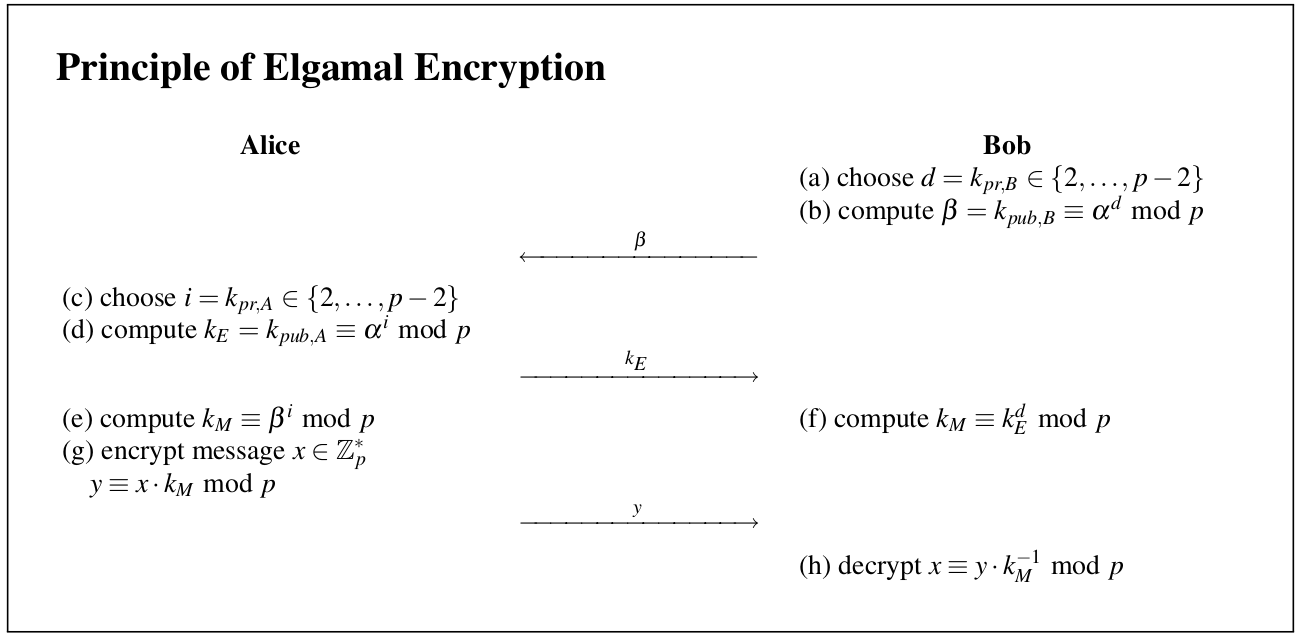
\includegraphics[scale=0.35]{ElGamalPrinciplePaar.png}
	\centering
\end{figure}

This protocol is similar to Diffie-Hellman: the private and public keys of Bob are computed the same way, and do not change over time, however Alice has to generate a new pair for the encryption of every message.

The key $k_E$ is \textbf{ephemeral}, meaning that it only exists temporarily, and $k_M$ is the joint key for masking the plain text. To encrypt a message, Alice multiplies the plaintext message $x$ by $k_M$ and Bob reverses this operation using the inverse mask.

\subsection{Protocol}
ElGamal encryption method works thanks to an important property of cyclic groups: given $k_M \in \mathbb{Z}^*_p$, every message $x$ maps to another cipher text computing $k_M \cdot x$, and random values allow to obtain the \textit{same probability} for every cipher text. 

\begin{figure}[h]
	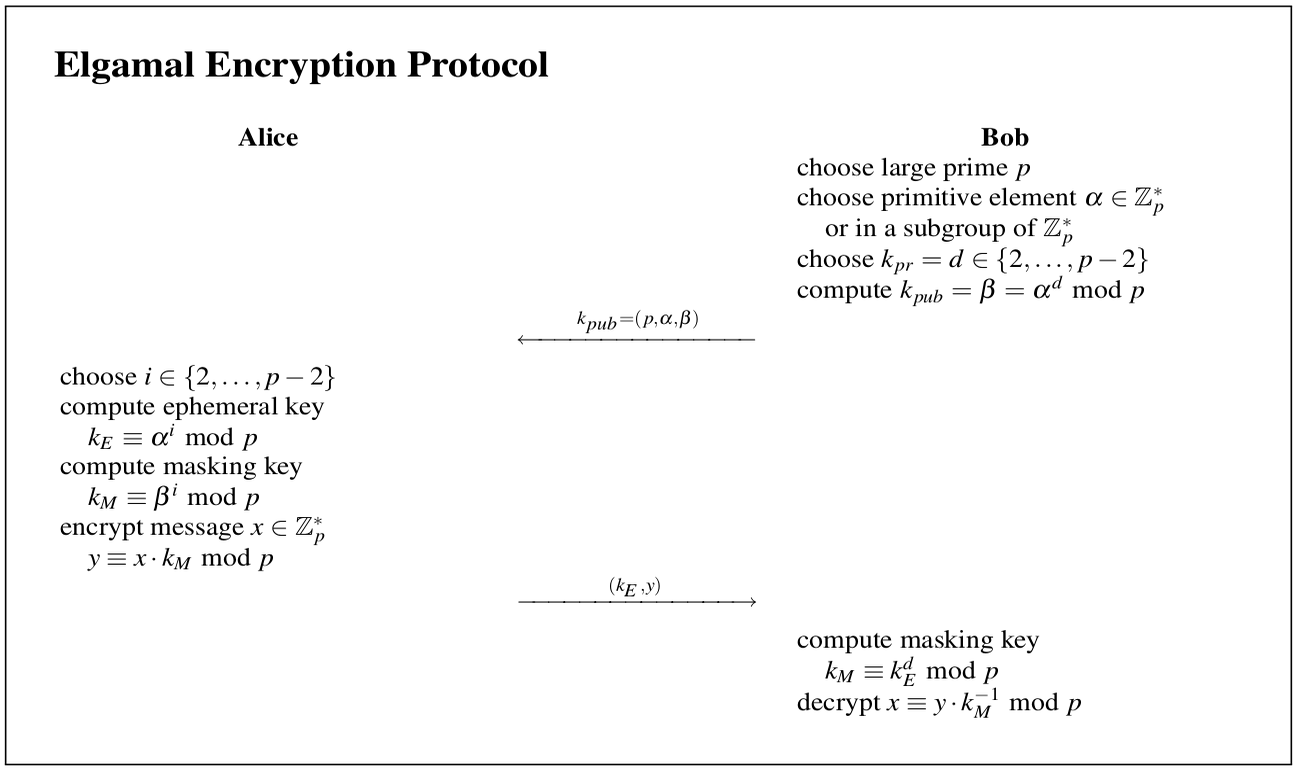
\includegraphics[scale=0.35]{ElGamalProtocolPaar.png}
	\centering
\end{figure}

The actual protocol is composed by three phases: \textbf{setup}, \textbf{encryption} and \textbf{decryption}. It starts by fixing a very large finite field $\mathbb{Z}^*_p$ and an element $\alpha \in \mathbb{Z}^*_p$ (preferably, but not necessarily a generator). 

Supposing an use of plain text message units with numerical equivalents in $\mathbb{Z}^*_p$, each user $A$ randomly chooses an integer $i$ in the range $0 < i < p - 1$. This integer $i$ is the secret deciphering key, while the public enciphering key is the element $k_E = \alpha^i \in \mathbb{Z}^*_p$.	

To send a message $y$ to the user $A$, an integer $d$ is chosen at random, and $A$ is sent the pair of elements:
$$(\alpha^d, y\alpha^{id})$$
$\alpha^{id} = k_E^d$ can be computing without knowing $i$ simply by raising $\alpha$ by the $d$-th power. Now Alice, who is aware of $i$, can recover $y$ from this pair simply by raising the first element $\alpha^d$ to the $i$-th power and dividing the result by the second element.

Public keys can be obtained in any way, for instance from key servers or unencrypted means. There is no security issues involved in this transmission, as the only secret is the exponent and therefore computationally infeasible.

In other words, the message is being masked but also contains a way to be recovered only by someone knowing the initial value $i$. 

The Diffie-Hellman sequence of operations is rearranged, since Bob receives only one message from Alice containing the ephemeral key and the encrypted text. In this case, however, the couple $(k_E, y)$ is generally \textbf{twice as long} as the message, since parameters have a bit length of $\lceil\log_2p\rceil$.

\subsubsection{Example}
Alice wants to send the message $x = 26$.

Bob generates $p = 29$ and $\alpha = 2$, then chooses $k_{pr, B} = d = 12$ to compute $\beta = \alpha^d \equiv 7 \mod 29$.

Alice receives the triple $k_{pub, B} = (p, \alpha, \beta) = (29, 2, 7)$, chooses $i = 5$ and then uses those to obtain the two temporary keys:
\begin{enumerate}
	\item $k_E = \alpha^i \equiv 3 \mod 29$
	\item $k_M = \beta^i \equiv 16 \mod 29$
\end{enumerate}
Alice encrypts $y = x \cdot k_M \equiv 10 \mod 29$, and sends it to Bob with the ephemeral key $k_E$.

Bob computes $k_M = k_E^d \equiv 16 \mod 29$, which is the same as Alice, and uses it to decrypt the message:
$$x = y \cdot k^{-1}_M \equiv 10 \cdot 20 \equiv 26 \mod 29$$

\subsection{Proof}
Assuming the value $d_{k_{pr}}(k_E, y)$ actually returns the original message $x$:
\begin{equation}
\begin{split}
d_{k_{pr}}(k_E, y) &\equiv y \cdot (k_M)^{-1} \mod p \\
&\equiv [x \cdot k_M] \cdot (k_E^d)^{-1} \mod p \\
&\equiv [x \cdot (\alpha^d)^i]^{-1} \mod p \\
&\equiv x \cdot \alpha^{d \cdot i - d \cdot i} \mod p \\
&\equiv x \mod p
\end{split}
\end{equation}

\subsection{Practical applications}
ElGamal encryption is not widely used in practice, since one of the best known practices to break it exploits its malleability: the ciphertext $(k_E, y)$ can be replaced with $(k_e, sy)$ for some integer $s$.

The receiver therefore then computes:
\begin{equation}
\begin{split}
d_{k_{pr}}(k_E, sy) &\equiv sy \cdot (k_M)^{-1} \mod p \\
&\equiv s \cdot (x \cdot k_M) \cdot k_M^{-1} \mod p \\
&\equiv sx \mod p
\end{split}
\end{equation}

The decrypted text is also a multiple of $s$, and although an attacker would not be able to decrypt the message, he is able to manipulate it for instance doubling or tripling the value of the result and compromising communication.

The ElGamal encryption system is used in GNU Privacy Guard System and recent versions of PGP. 

GnuPG implementation, however, until late 2003 had an insecure algorithm whose private exponent was too short and thus easy to break. All signatures created before then are considered compromised. 

\subsubsection{Computational aspects}
As previously stated, the ciphertext is twice as long as the message: therefore, the message expansion factor of ElGamal is two. 

Furthermore, it is a \textbf{probabilistic encryption scheme}: encrypting two identical messages $x_1, x_2 \in \mathbb{Z}^*_p$ using the same public key results with \textit{extremely high likelihood} in two different ciphertexts $y_1 \neq y_2$. 

This happens since $i$ is chosen at random from $\{2, 3, \dots, p - 2\}$ every time a message is encrypted, causing the session key $k_M = \beta^i$ to also be random. This is an effective method to prevent brute-force attacks.

Key generation involves finding a prime number $p$, which needs to have a length of at least 1024 bits and can be found through one of the prime-finding algorithms. 

The public key can easily be computed using the square-and-multiply algorithm, since it requires exponentiation operations.

This is also applied to the encryption procedure: it involves two modular exponentiations and one modular multiplication, all operands having a bit length of $\lceil\log_2p\rceil$. Since exponentiations are independent from the plain text, they can be calculated in advance and stored to be retrieved when actual encryption is needed, to reduce the total time.

Decryption is performed again through the exponentiation $k_M = k^d \mod p$, using square-and-multiply, followed by an inversion performed with extended Euclidean algorithm.

\textbf{Fermat's Little Theorem }allows to combine steps, using the following property:
$$k_E^{p-1} \equiv 1 \mod p \qquad \forall\ k_E \in \mathbb{Z}^*_p$$

Decryption can be performed as:
\begin{equation}
\begin{split}
k_M^{-1} &\equiv (k_E^d){-1} \mod p \\
&\equiv (k_E^d){-1}\cdot k_E^{p-1} \mod p \\
&\equiv k_E^{p-d-1} \mod p
\end{split}
\end{equation}
This equivalence relation allows to compute the inverse of the masking key using only a single exponentiation with $p - d - 1$, which is essentially one execution of square-and-multiply.

After that, one modular multiplication is required to recover $x \equiv y \cdot k_M^{-1} \mod p$. 

\subsubsection{Security}
To analyse the security of ElGamal, firstly an assumption must be introduced, consisting in the \textbf{Decisional Diffie-Hellman}. This assumption states that, considering a group $G$ and a generator $a$, given $x, y \in \mathbb{Z}^*_q$, the value $a^{xy}$ looks like a generic random element.

This can also be stated imposing that the probability distributions $(a^x, a^y, a^{xy})$ and $(a^x, a^y, a^z)$, with $x, y, z \in \mathbb{Z}^*_q$ randomly and independently chosen, are computationally indistinguishable. 

Decisional Diffie-Hellman is a stronger assumption than just discrete logarithm, since it forbids computing discrete logarithms of $a^x$ and $a^y$ separately to then combine them and cracking $a^{xy}$. 

The security of ElGamal can be further assessed distinguishing between two kinds of attacks:
\begin{itemize}
	\item Passive, which are listen-only;
	\item Active, which allow an attacker to generate and alter messages.
\end{itemize}

Passive attacks consist in retrieving the message $x$ from the information $p, \alpha, \beta = \alpha^d, k_E = \alpha^i$ and $y = \beta^i$ obtained by eavesdropping the channel. 

Currently, there is no method to solve Diffie-Hellman protocol other than computing discrete logarithms, therefore the most efficient way to avoid that is choosing strong keys. In fact, the only ways an attacker can break the ElGamal scheme are:
\begin{enumerate}
	\item Finding $d$, i.e.\ computing $d = \log_\alpha \beta \mod p$, which is computationally infeasible;
	\item Trying to guess the random exponent $i = log_\alpha k \mod p$, which still involves solving the discrete logarithm problem.
\end{enumerate}
The index-calculus algorithm can be used in both cases, thus in order to guarantee security of ElGamal, $p$ should be at least of 1024 bits and $\alpha$ has to be a primitive element. 

Active attacks compromise the authenticity of public keys, having them belong to an untrusted third party. This can be prevented using certificates or digital signatures.

Another pitfall is that the random exponent $i$ \textbf{should not be reused}: assuming Alice uses the same value for the encryption of two subsequent messages $x_1$ and $x_2$, then the two masking keys would be the same, namely $k_M = \beta^i$, along with the ephemeral keys.

Two identical cyphertexts $(y_1, k_E)$ are therefore sent through the channel. If an attacker can guess the first message, the second one can be computed as well using the masking key $k_M \equiv y_1x_1^{-1} \mod p$ since $x_2 \equiv y_2k_M^{-1} \mod p$.

This consequently works for every text encrypted with the same $i$. Furthermore, an attacker knows that $i$ is being reused, since it leads to the same ephemeral key. As a consequence, the secret exponent must not be repeated, choosing different seeds for picking random numbers. 

	\section{Algorithms}
Defining algorithms to find the discrete logarithm in finite fields can be done supposing that all the prime factors of $n - 1$ are small, without loss of generality. This allows to assume fast algorithms exist, using $\mathbb{Z}^*_n$ as field.

As from today, one of the best results in computing was achieved in 2019 by a group of researchers who announced the computation of the discrete logarithm of the number (RSA-240 + 49204), composed by 795 bit. This was obtained using a 2.1GHz CPU and took approximately 4000 core-years.

There are also reports of computing a discrete logarithm within a 768-bit prime field, taking 5300 core years, using the same algorithm as the previous (Number Field Sieve).

\subsection{Silver, Pohlig and Hellman algorithm}
The Silver-Pohlig-Hellman algorithm exploits a possible factorization of the order of a group through the \textbf{Chinese Remainder Theorem}. 

This applies to groups whose order is either a smooth integer or a prime power, iteratively computing the digit of the discrete logarithm by shifting out all but one unknown digit in the exponent.

The prime factorization of a group with order $|G|$ can be written using its $p$-th roots as:
$$|G| = p_1^{e_1} \cdot p_2^{e_2} \cdot \dots p_l^{e_l}$$
Computing the discrete logarithm $x = \log_\alpha \beta$ in $G$ can be performed through a \textbf{divide-and-conquer} approach, finding smaller discrete logarithms $x_i \equiv x \mod p_i^{e_i}$ in the subgroups of order $p_i$ through some attack such as Pollard's method.

Then, all $x_i$ are used applying the Chinese Remainder Theorem, determining an unique $x$ thanks to pairwise co-prime divisors. 

A consequence of the properties of prime factors is that one needs to know the factorization of the group order, which is not always easy.

\subsection{Index-calculus algorithm}
The index-calculus \textbf{probabilistic} algorithm has the particularity of working only under certain assumptions, such as cyclic groups $\mathbb{Z}^*_p$ and $GF(2^m)$, and has a lot in common with integer factorization although generally uses polynomials in rings. 

However, it is one of the most efficient ways to compute discrete logarithm, due to its \textit{high parallelism} involving operations independent from one another. 

Here, the term \textbf{index} is a commonly used word to define the discrete logarithm: $x = ind(a) \mod q$ for some base $b$, for $b^x \equiv a \mod m$ if $b$ is a primitive root of $q$ and $\gcd(a, q) = 1$.

Index-calculus depends on the property that a significant fraction of elements of $G$ can be efficiently expressed as \textbf{products of elements} of a small subset of $G$, assuming $|G|= q = p^n$ is a fairly large power of a small prime $p$. 

This algorithm allows to find for any $x \in \mathbb{Z}^*_q$ the value of $x \mod q - 1$ such that $y = \alpha^x$, with $\alpha$ generator.

It works in two phases: the first one consists in precomputation, since it does not depend on the element $x$ to decrypt, and only has to be carried once. An irreducible element $f \in \mathbb{Z}^*_q$ is identified, and a subset $B \subset \mathbb{Z}^*_q$ is chosen, which will serve as ``basis'' and usually consists of all monic irreducible polynomials of arbitrary degree. 

Then, all discrete logarithms f $a \in B$ are computed, i.e.\ a random integer $t \in [1, q - 2]$ is chosen and then $b^t$ is computed through repeated squaring. The algorithm finds all elements $c \in \mathbb{Z}^*_q$ such that:
$$c = b^t \mod f$$

Now, the index-calculus algorithm attempts to write $c$ as:
$$c = c_0 \prod_{a \in B} a ^{m}$$
$m$ is the highest power of $a$ which divides $c$. One way to determine this is to run through all $a \in B$ and divide $c$ successively by $a^m$. If the constant $c_0$ is the only one remaining after the division, then $c$ has the above form; otherwise, a different random integer $t$ is chosen.

Another good method to compute $c$ as products of elements $a \in B$ is using an \textit{integer factorization algorithm}, hence the close relation between these two problems.

Now, supposing some $c \equiv b^t \mod f$ has been found, and $c$ has the desired type of factorization, taking the discrete logarithm of both sides allows to obtain:
$$ind(c) - ind(c_0) \equiv \sum_{a \in B} m \cdot ind(a) \mod q - 1$$
The \textbf{modulo} operation is introduced since the discrete logarithm is only defined modulo $q - 1$. The left side of the equivalence is known, since $ind(c) = t$, and discrete logarithms of constants are assumed to be known as well.

The coefficients $m$ are also known, leaving only values $ind(a)$ and $a \in B$ to be found. 

Assuming $|a| = h$, unknowns can be obtained through a linear system of equations with $h$ unknowns. Supposing integers $t$ can be chosen until a large number of different $c$ which factor into a product of $a$, eventually $h$ \textbf{independent} congruences will be found, written as:
$$t = ind(c_0) \equiv \sum_{a \in B} m \cdot ind(a) \mod q - 1$$
Here, \textit{independent} implies that the determinant of the coefficient matrix $\{m\}$ is prime to $q - 1$.

The system of unknowns can then be solved, completing the first stage of index-calculus. Precomputation gives a large set of all the discrete logs of $a \in B$, from which to calculate any other discrete log.

The final stage is performed supposing $x$ is the message whose discrete logarithm should be computed, and that the previous phase has already given all values of $ind(a),\ \forall\ a \in B$.

A random integer $t$ is once again chosen, and $y = xb^t$ is computed, i.e.\ the unique element $y \in \mathbb{Z}^*_q$ satisfying $y \equiv xb^t \mod f$.

As in the first stage, $y$ has to be factored into a constant $y_0$ times the product of powers of $a$, with $a \in B$. If not, another $t$ is picked, and so on, until an integer is obtained such that:
$$y = y_0 \prod_{a \in B} a ^{m}$$

As soon as this happens, the algorithm can terminate:
$$ind(x) = ind(y) - t \qquad \and \qquad ind(y) = ind(y_0) + \sum_{a \in B} m \cdot ind(a)$$
All the terms are known, therefore a message can be decrypted. Furthermore, advances in research have significantly sped up the process in finding discrete logs.

This algorithm allows to obtain a runtime which is not exponential in the bit length of the order, but \textbf{subexponential}. This can once again be compared to integer factorization: the order of magnitude of time needed to solve the discrete log problem for $q = p^n$ which is $k$ bits long is the same as factoring a $k$-bit number. 

In order to provide a security of 80 bits, an attacker has thus to perform $2^{80}$ steps, therefore the prime $p$ of a discrete logarithm in $\mathbb{Z}^*_p$ should be at least 1024 bit long; for $GF(2^m)$, index-calculus is even more powerful, making these groups \textit{unusable} in practice.

\subsection{Number Field Sieve}
The Number Field Sieve algorithm, based on index-calculus, is currently the fastest known algorithm for finding both discrete logarithms and \textit{integer factoring}, and the method used to break the record on the 795-bit value previously mentioned. 

The key idea of the Number Field Sieve, starting from integer factorization consists in \textbf{iteratively finding divisors within a field}. Assuming $q$ is a composite number, the algorithm generates pairs such that:
$$x \equiv y \mod q$$

$\gcd(x - y, q)$ is a non-trivial divisor of $q$ with probability 0.5, and after finding several pairs, $q$ can be factorized.

The previous equation can also be stated including prime numbers $p_i$ and their power within the factorization, i.e.:
$$x = p_1^{n_1} \cdot p_2^{n_2} \cdot \dots \cdot p_m^{n_m}$$

This approach is used while computing discrete logarithm: when enough elements have been found, the linear system of equations is solved, and the logarithm is consecutively applied such that $\log(p_i) = a_i$. Therefore, if some element $b$ can be expressed as $b = p_1^{n_1} \cdot p_2^{n_2} \cdot \dots \cdot p_k^{n_k}$, then its discrete logarithm consists in:
$$\log(b) = n_1\log(p_1) \cdot n_2\log(p_2) \cdot \dots \cdot n_k\log(p_k)$$

Given integers $a$ generator of $\mathbb{Z}^*_q$, $b$, $n$ and a prime number such that $p^q = n$, $x$ solving $a^x \equiv b \mod q$, the algorithm attempts to find two monic polynomials $y_1$ and $y_2$ having the property:
$$y_1 \equiv 0 \mod p \qquad \land \qquad y_2 \equiv 0 \mod p$$

Denoting with $\lambda_i \in \mathbb{C}$ the root of $y_i$, then holds that $y_i$ is the minimal polynomial of $\lambda_i$ and it is possible to define fields in which it is ensured the unique factorization.

Having $y_i(\lambda_i) = 0$, then it is again possible to express $y_i$ as a combination of powers which can be used to reduce polynomials and define their complex product within the algebraic \textit{number complex field}. This can be mapped to the original field, while trying to compute couples of integer values which are squares of another number, to also be able to factorize in $\mathbb{Z}^*_q$.

The system obtained with all the factors is then solved, usually using the Chinese Remainder Theorem.  



	\section{Other attacks}
Attacks against discrete logarithm involve finding the integer $x$ for a given $\alpha$ and $\beta$ in $G$ such that:
$$\beta = \alpha \circ \alpha \circ \dots \circ \ alpha = \alpha^x$$

In 1997, a lower bound for discrete logarithms was given: any generic algorithm that solves with high probability the problem must perform at least $\Omega(p^{1/2})$ group operations, where $p$ is the largest prime dividing the cardinality of the group. The same result holds for non cyclic groups and Diffie-Hellman protocol.

The exact difficulty of computing this is still unknown: despite the existence of algorithms, there could be better or more powerful ones which still are undiscovered (similarly to integer factorization). 

Generic algorithms are methods which only rely on the group operation $\circ$, without needing further algebraic structure. This property makes them applicable in any cyclic group.

\subsection{Brute force search}
Brute-force is the most naive and costly generic algorithm to obtain the discrete logarithm $\log_\alpha\beta$: all powers of the generator $\alpha$ are computed \textbf{successively}, until the result equals $\beta$.

For a random logarithm $x$, on average the correct solution is expected to be found after checking \textit{half of the possible values}. This gives a complexity of $O(|G|)$, linear in the cardinality of the group.

To avoid this kind of attack to be successful, therefore, the cardinality of groups must be sufficiently large, without any other particular measure. 

In the case of $\mathbb{Z}^*_p$ with $p$ prime, approximately $\frac{p-1}{2}$ tests are required to compute the discrete logarithm, meaning that $|G| = p - 1$ should be in the order of at least $2^{80}$ to make a brute force infeasible using the modern hardware.

\subsection{Shank's method}
Shank's method is another generic algorithm which allows to reduce the time of a brute force search, at the trade off of occupying more storage. It is a meet-in-the-middle attack, storing intermediate values by trying to successively crack the multiple steps of discrete logarithm encryption.

The procedure is based on rewriting the discrete logarithm in a two-digit representation:
$$x = x_gm = x_b \qquad 0 \leq x_g, x_b < m$$
The value $m$ is chosen to be approximately the square root of the cardinality of the set, i.e.\ $m = \lceil{\sqrt{|G|}}\rceil$. Discrete logarithm can then be stated as $\beta = \alpha^x = \alpha^{x_gm + x_b}$ which leads to:
$$\beta \cdot (\alpha^{-m})^{x_g} = \alpha^{x_b}$$ 
The core idea of the algorithm is using a divide-and-conquer approach to find $x_a$ and $x_b$ separately, in two phases:
\begin{enumerate}
	\item Baby-step, where all the values $\alpha^{x_b}$ with $0 \leq x_b < m$ are computed and stored with approximately $m \approx \sqrt{|G|}$ operations;
	\item Giant-step, in which the program checks for all $x_g$ in $0 \leq x_g < m$ whether this condition is fulfilled: 
	$\beta \cdot (\alpha^{-m})^g \stackrel{?}{=} \alpha^{x_b}$ for some stored entry $\alpha^{x_b}$ that was computed during the previous step.
\end{enumerate}
In case of a match, i.e.\ $\beta \cdot (\alpha^{-m})^{x_g, 0} = \alpha^{x_b, 0}$ for some pair $(x_{g, 0}, x_{b, 0})$ the discrete logarithm is:
$$x = x_{g, 0}m + x_{b, 0}$$
Further speed up the method can be obtained using efficient lookup schemes, such as \textbf{hash tables} which allow constant time search.

This algorithm has a total computational time and space of $O(\sqrt{|G|})$, which means that in a group of order $2^{80}$ an attacker would approximately need $2^{40}$ operations, easily obtainable with modern hardware.

Direct consequence of this is that groups need to have a cardinality of at least $|G| \geq 2^{160}$, to make Shank's method have a complexity of $2^{80}$ and therefore be infeasible. In case of prime groups $G = \mathbb{Z}^*_p$, $p$ must have a length of at least 160 bit; using prime groups is advised since otherwise Shank's method would have an even smaller complexity. 

\subsection{Pollard's Rho method}
Pollard's Rho method has the same computational time as Shank's algorithm, yet constant space requirements. It is based on the \textbf{birthday paradox}, concept related to the higher likelihood of collisions found between random attack attempts and a fixed degree of permutations.

The basic idea consists in pseudo-randomly generate ($\rho$ represents randomness) group elements of the form $\alpha^i \cdot \beta^j$, keeping track of values $i$ and $j$, to then continue until obtaining a collision:
$$\alpha^{i_1} \cdot \beta^{j_1} = \alpha^{i_2} \cdot \beta^{j_2}$$
Substituting $\beta = \alpha^x$ and comparing the exponents on both sides of the equation, the collision leads to the following formula:
$$i_1 + xj_1 \equiv i_2 + jx_2 \mod |G| \qquad \rightarrow \qquad x \equiv \frac{i_2 - i_1}{j_1 - j_2} \mod |G|$$ 
The second part allows to find the discrete logarithm. Furthermore, additional methods to speed up computations such as the Extended Euclidean Algorithm and Floyd's cycle-finding algorithm.

Its computational time is approximately $O(\sqrt{n})$, while used together with Silver-Pohlig-Hellman it can achieve $O(\sqrt{p})$ where $p$ is the largest prime factor of $n$.

The practical importance of Rho's method is it being the best-known algorithm in \textit{elliptic curve group}s, making 160 bit operands very popular within this cryptography; however, it is not the most powerful attack for discrete logarithm and it does not work well in a distributed environment.



	\section{Comparison with integer factorization}
While computing discrete logarithms within a field and computing the integer factorization of a composite number are distinct problems, they share some characteristics:
\begin{itemize}
	\item Both concern cases of the small subgroup problem for finite commutative groups;
	\item Both are NP-hard problems, despite the existence of efficient algorithms on quantum computers;
	\item Both have been extensively used to construct strong encryption systems still valid today.
\end{itemize}

Furthermore, some algorithms to break integer factorization also have practical application in solving discrete logarithms, such as index-calculus. Shank and Pollard, on the other hand, have both developed different methods to solve the two problems.

Solving the discrete logarithm problem would actually solve the integer factorization problem, and vice versa, for the two following reasons:
\begin{enumerate}
	\item One system can be reduced to the other, since they both work on groups using the modulo operation;
	\item Both are assumed to be in the same computation class of NP, therefore solving any NP-hard problem would imply there exist an efficient way to consequently solve all the others.
\end{enumerate}

Since the RSA cryptography extensively rely on integer factorization, it is considered equally hard to break as the discrete logarithm. Both algorithms, therefore, are considered strong enough for safe encryption purposes and have similar performance.

The nature of Diffie-Hellman, however, makes it susceptible to man-in-the-middle attacks, since it does not authenticate involved parts during the exchange and requires additional confirmation.

RSA, on the other hand, allows digital signatures, although still needs the exchange of a public key beforehand. 

\section{Final considerations}
Discrete logarithm has been proved to be secure against both active and passive attacks: the only effective way to break this problem would be to come up with new algorithms, since the key length can be arbitrarily increased to resist modern hardware. 

However, there are some problems:
\begin{itemize}
	\item Is Decisional Diffie-Hellman equally hard as discrete logarithm, when dealing with preprocessing attacks?
	\item Is quantum computing an efficient way to reduce computational time?
	\item Would attacks on elliptic curves also influence discrete logarithm?
\end{itemize}

Having these open questions allow space for urther research and development, while still ensuring computation infeasibility. 
	\clearpage
\begin{thebibliography}{}
	\footnotesize
	
	\bibitem{koblitz}
	N. Koblitz - A Course in Number Theory and Cryptography
	
	\bibitem{knuth}
	D. Knuth - The Art of Computer Programming, Vol. II
	
	\bibitem{paar}
	C. Paar, J. Pelzl - Understanding Cryptography
	
	\bibitem{shor}
	P. W. Shor - Polynomial-Time Algorithms for Prime Factorization and Discrete Logarithms on a Quantum Computer
	
	\bibitem{ike}
	\href{https://tools.ietf.org/html/rfc2409}{https://tools.ietf.org/html/rfc2409}
	
	\bibitem{2019}
	\href{https://listserv.nodak.edu/cgi-bin/wa.exe?A2=NMBRTHRY;fd743373.1912}{https://listserv.nodak.edu/cgi-bin/wa.exe?A2=NMBRTHRY;fd743373.1912}
	
	\bibitem{european}
	P. Horster, H Knoblock - Discrete Logarithm Based Protocols
	
	\bibitem{bdcalc}
	\href{https://www.di-mgt.com.au/solving-discrete-logarithm-problem.html}{https://www.di-mgt.com.au/solving-discrete-logarithm-problem.html}
	
	\bibitem{shoup}
	V. Shoup - Lower Bounds for Discrete Logarithms and Related Problems
	
	\bibitem{768}
	T. Kleinjung, C. Diem, A. Lenstra, C. Priplata, C. Stahlke - Computation of a 768-bit prime field discrete logarithm
	
	\bibitem{tls}
	D. Adrian et al. - Imperfect Forward Secrecy:How Diffie-Hellman Fails in Practice
	
	\bibitem{tum}
	A. Meier - The ElGamal Cryptosystem
	
	\bibitem{theorydish}
	\href{https://theorydish.blog/2018/01/24/preprocessing-attacks-on-the-discrete-log-problem/}{https://theorydish.blog/2018/01/24/preprocessing-attacks-on-the-discrete-log-problem/}
		
\end{thebibliography}
	
\end{document}

% todo:
% teoremi nei blocchi?

% first DL, then DH, then elgamal, then maths and algorithms
% always have practical components (real threat, practical part)
% add a bit of practice: is this just theoretical or something we need in practice?
% why is elgamal not widely used?

% google scholar
% divide last section in respective part (add computational aspects in each topic)

% in the presentation, choose 1 attack and 1 algorithm
% schould be around 15 pages, not more than 20

% send the updated table of contents in the next two weeks
% add technical things: 
% find a way to include audience, to figure out if they are listening, ask questions
% get feedback!


	